\section{Vorwort}
\subsection{Problemstellung}

Auf dem Markt existieren schon alle möglichen Bewässerungssysteme. Von Rasenbewässerungen bis zu Topfpflanzen ist alles vertreten. Die meisten Systeme existieren für die Gartenbewässerung (zum Beispiel von Gardena) und werden an
die Wasserleitung mit 1/2 Zoll direkt angeschlossen. Die Steuerungen sind eher einfach gehalten. Einstellbar sind die Wassermenge und die Bewässerungszeitpunkte. Bei den Lösungen für Beete und Kübel ist eine Steuerung eher selten. Sie erfolgt
durch das Auf- und Zudrehen der Wasserzufuhr. Aus dieser Marktlage folgernd, wird in diesem Projekt ein Bewässerungssystem für Topf- und Beetpflanzen geplant und realisiert.

\subsection{Projektziel}
Das System soll eine Regelung enthalten, die mindestens dieselben Funktionen enthalten soll, wie die bereits bestehenden Produkte. Zusätzlich soll durch  ein oder zwei Feuchtigkeitssensoren die Feuchtigkeit in die Steuerung einfließen
und somit zur Regelung wird. Die Wasserzufuhr soll wahlweise über ein separates Wasserreservoir oder über einen Standardwasseranschluss zur Verfügung gestellt werden. Die gemessenen Daten werden in einem Arduinoboard, welches die
zentrale Mikrocontrollereinheit ist, zusammengeführt und ausgewertet. Die Daten und Änderungen im Bewässerungszyklus können über eine Wlanschnittstelle entnommen und verändert werden. Die Schnittstelle wird über ein ESPboard realisiert.
Die Kosten der Materialen soll um 200 \euro{} liegen.

\section{Aufgabenteilung}
Das Projektteam besteht aus vier Mitarbeitern. Es sind dementsprechend vier Aufgabengebiete erstellt worden. Das erste Gebiet umfasst den Aufbau und die Implementierung der Sensoren. Hierfür verantwortlich ist Dennis Hufnagel.
Der nächste Bereich ist die Wasser- und Stromversorgung. Dort ist Silas Leidel verantwortlich. Den dritten Bereich, welcher die Realisation der Steuerung im Arduino umfasst, betreute Marcel Fuchs. Die WLAN-Schnittstelle und
die Konfiguration des ESPboards übernimmt Michael Kainz.

\begin{figure}[ht]
    \centering
    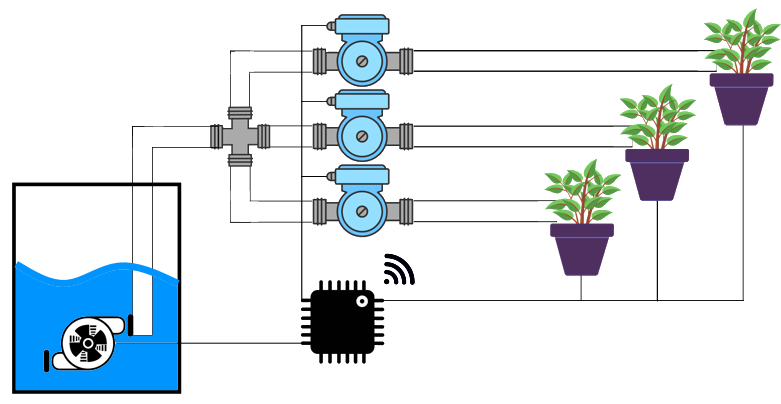
\includegraphics[width=\textwidth]{silas/blockschaltbild}
    \caption{Schema der Anlage}
\end{figure}